\documentclass[11pt]{article}
% https://www.gradescope.com/help#help-center-item-answer-formatting-guide
\usepackage{microtype}
\usepackage{graphicx}
\usepackage{wrapfig}
\usepackage{url}
\usepackage{wrapfig}
\usepackage{color}
\usepackage{marvosym}
\usepackage{enumerate}
\usepackage{subfigure}
\usepackage{tikz}
\usepackage[fleqn]{amsmath}
\DeclareMathOperator*{\argmax}{argmax}
\DeclareMathOperator*{\argmin}{argmin}
\usepackage{amssymb}
\usepackage{hyperref}
\usepackage[many]{tcolorbox}
\usepackage{lipsum}
\usepackage{float}
\usepackage{trimclip}
\usepackage{listings}
\usepackage{environ}% http://ctan.org/pkg/environ
\usepackage{wasysym}
\usepackage{array}
\usepackage{bbm}
\usepackage{enumitem}
\usepackage{tikz}
\usetikzlibrary{shapes, arrows, calc, positioning,matrix}
\tikzset{
data/.style={circle, draw, text centered, minimum height=3em ,minimum width = .5em, inner sep = 2pt},
empty/.style={circle, text centered, minimum height=3em ,minimum width = .5em, inner sep = 2pt},
}
\newcommand{\ztnodesize}{.6}
\newcommand{\factorsize}{1}
\newcommand{\nodesize}{1.3}

\oddsidemargin 0mm
\evensidemargin 5mm
\topmargin -20mm
\textheight 240mm
\textwidth 160mm

\newcommand{\vwi}{{\bf w}_i}
\newcommand{\vw}{{\bf w}}
\newcommand{\vx}{{\bf x}}
\newcommand{\vy}{{\bf y}}
\newcommand{\vxi}{{\bf x}_i}
\newcommand{\yi}{y_i}
\newcommand{\vxj}{{\bf x}_j}
\newcommand{\vxn}{{\bf x}_n}
\newcommand{\yj}{y_j}
\newcommand{\ai}{\alpha_i}
\newcommand{\aj}{\alpha_j}
\newcommand{\X}{{\bf X}}
\newcommand{\Y}{{\bf Y}}
\newcommand{\vz}{{\bf z}}
\newcommand{\msigma}{{\bf \Sigma}}
\newcommand{\vmu}{{\bf \mu}}
\newcommand{\vmuk}{{\bf \mu}_k}
\newcommand{\msigmak}{{\bf \Sigma}_k}
\newcommand{\vmuj}{{\bf \mu}_j}
\newcommand{\msigmaj}{{\bf \Sigma}_j}
\newcommand{\pij}{\pi_j}
\newcommand{\pik}{\pi_k}
\newcommand{\D}{\mathcal{D}}
\newcommand{\el}{\mathcal{L}}
\newcommand{\N}{\mathcal{N}}
\newcommand{\vxij}{{\bf x}_{ij}}
\newcommand{\vt}{{\bf t}}
\newcommand{\yh}{\hat{y}}
\newcommand{\code}[1]{{\footnotesize \tt #1}}
\newcommand{\alphai}{\alpha_i}
\newcommand{\defeq}{\overset{\text{def}}{=}}
\renewcommand{\vec}[1]{\mathbf{#1}}



\bgroup
\def\arraystretch{1.5}
\newcolumntype{x}[1]{>{\centering\arraybackslash\hspace{0pt}}p{#1}}
\newcolumntype{z}[1]{>{\centering\arraybackslash}m{#1}}

%Arguments are 1 - height, 2 - box title
\newtcolorbox{textanswerbox}[2]{%
 %width=\textwidth,
 colback=white,colframe=blue!30!black,floatplacement=H,height=#1,title=#2,clip lower=true,before upper={\parindent0em}}

 \newtcolorbox{eqanswerbox}[1]{%
 width=#1,colback=white,colframe=black,floatplacement=H,height=3em,sharp corners=all,clip lower=true,before upper={\parindent0em}}

 %Arguments are 1 - height, 2 - box title
 \NewEnviron{answertext}[2]{
        \noindent
        \marginbox*{0pt 10pt}{
        \clipbox{0pt 0pt 0pt 0pt}{
        \begin{textanswerbox}{#1}{#2}
        \BODY
        \end{textanswerbox}
        }
        }
}

%Arguments are 1 - height, 2 - box title, 3 - column definition
 \NewEnviron{answertable}[3]{
        \noindent
        \marginbox*{0pt 10pt}{
        \clipbox{0pt 0pt 0pt 0pt}{
        \begin{textanswerbox}{#1}{#2}
                \vspace{-0.5cm}
                        \begin{table}[H]
                        \centering
                        \begin{tabular}{#3}
                                \BODY
                        \end{tabular}
                        \end{table}
        \end{textanswerbox}
        }
        }
}

 %Arguments are 1 - height, 2 - box title, 3 - title, 4- equation label, 5 - equation box width
 \NewEnviron{answerequation}[5]{
        \noindent
        \marginbox*{0pt 10pt}{
        \clipbox{0pt 0pt 0pt 0pt}{
        \begin{textanswerbox}{#1}{#2}
                \vspace{-0.5cm}
                        \begin{table}[H]
                        \centering
                \renewcommand{\arraystretch}{0.5}% Tighter

                        \begin{tabular}{#3}
                                #4 =    &
                        \clipbox{0pt 0pt 0pt 0pt}{

                        \begin{eqanswerbox}{#5}
                                $\BODY$
                        \end{eqanswerbox}
                        } \\
                        \end{tabular}
                        \end{table}

        \end{textanswerbox}
        }
        }
}

 %Arguments are 1 - height, 2 - box title
 \NewEnviron{answerderivation}[2]{
        \noindent
        \marginbox*{0pt 10pt}{
        \clipbox{0pt 0pt 0pt 0pt}{
        \begin{textanswerbox}{#1}{#2}
        \BODY
        \end{textanswerbox}
        }
        }
}

\newcommand{\Checked}{{\LARGE \XBox}}%
\newcommand{\Unchecked}{{\LARGE \Square}}%
\newcommand{\TextRequired}{{\textbf{Place Answer Here}}}%
\newcommand{\EquationRequired}{\textbf{Type Equation Here}}%


\newcommand{\answertextheight}{5cm}
\newcommand{\answertableheight}{4cm}
\newcommand{\answerequationheight}{2.5cm}
\newcommand{\answerderivationheight}{14cm}

\newcounter{QuestionCounter}
\newcounter{SubQuestionCounter}[QuestionCounter]
\setcounter{SubQuestionCounter}{1}

\newcommand{\subquestiontitle}{Question \theQuestionCounter.\theSubQuestionCounter~}
\newcommand{\newquestion}{\stepcounter{QuestionCounter}\setcounter{SubQuestionCounter}{1}\newpage}
\newcommand{\newsubquestion}{\stepcounter{SubQuestionCounter}}


\lstset{language=[LaTeX]TeX,basicstyle=\ttfamily\bf}

\pagestyle{myheadings}
\markboth{Homework 5}{Spring 2020 CS 475/675 Machine Learning: Homework 5}

\title{CS 475 Machine Learning: Homework 5\\
Graphical Models, Inference, and Structured Prediction\\
Analytical Problems \\
\Large{Due: Saturday May 2, 2020, 11:59 pm}\\
40 Points Total \hspace{1cm} Version 1.0}
\author{YOUR\_NAME (YOUR\_JHED)}
\date{}

\begin{document}
\maketitle
\thispagestyle{headings}

\section*{Instructions }
We have provided this \LaTeX{} document for turning in this homework. We give you one or more boxes to answer each question.  The question to answer for each box will be noted in the title of the box.

 $\newline${\bf Other than your name, do not type anything outside the boxes. Leave the rest of the document unchanged.}

$\newline$\textbf{Do not change any formatting in this document, or we may be unable to
  grade your work. This includes, but is not limited to, the height of
  textboxes, font sizes, and the spacing of text and tables.  Additionally, do
  not add text outside of the answer boxes. Entering your answers are the only
  changes allowed.}


$\newline$\textbf{We strongly recommend you review your answers in the generated PDF to
  ensure they appear correct. We will grade what appears in the answer boxes in
  the submitted PDF, NOT the original latex file.}

\pagebreak

% \newquestion
% \section*{ Notation}
% {
% \begin{table}[h]
% % \caption{Notation.}\smallskip
% \centering
% \resizebox{.95\columnwidth}{!}{
% \smallskip\begin{tabular}{r l}
% \(\vec{x_i}\) & One input data vector. \(\vec{x_i}\) is \(M\) dimensional.
%                                     \(\vec{x_i} \in \mathbb{R}^{1 \times M}\).  \\ &
%                                     We assume $\vec{x_i}$ is augmented with a  $1$ to include a bias term. \\ \\
% \(\vec{X}\) &   A matrix of concatenated \(\vec{x_i}\)'s. There are \(N\) input vectors, so \(\vec{X} \in \mathbb{R}^{N \times M}\) \\ \\
% \(y_i\) & The true label for input vector \(\vec{x_i}\). In regression problems, \(y_i\) is a continuous value. \\ & In general \(y_i\) can be a vector, but for now we assume \(y_i\) is a scalar. \(y_i \in \mathbb{R}^1\). \\ \\

% \(\vec{y}\) &   A vector of concatenated \(y_i\)'s. There are \(N\) input vectors, so \(\vec{y} \in \mathbb{R}^{N \times 1}\) \\ \\

% \(\vec{w}\) & A weight vector. We are trying to learn the elements of \(\vec{w}\). \\ & \(\vec{w}\) is the same number of elements as \(\vec{x_i}\) because we will end up computing the dot product \(\vec{x_i} \cdot \vec{w}\). \\ & \(\vec{w} \in \mathbb{R}^{M \times 1}\). We assume the bias term is included in \(\vec{w}\). \\ \\
 
% % \(E_D(\vec{w})\) & The loss due to the model fit. \\ \\
% % \(E_\vec{w}(\vec{w})\) & The regularization term.  \\ \\

%  Notes: & In general, a lowercase letter (not boldface), $a$, indicates a scalar. \\
%   & A boldface lowercase letter, $\vec{a}$, indicates a vector. \\  &  A boldface uppercase letter, $\vec{A}$, indicates a matrix. \\
% \end{tabular}
% }
% \label{table2}
% \end{table}
% }

% %%%%%%%%%%%%%%%%%%%%%%%%%%%%%%%%%%%%%%%%%%%%%%%%%%%%%%%%%%%%%%%%%%%%%%%%%%%%%%%%
\newquestion
\section*{\arabic{QuestionCounter}) Probabilistic PCA (10 points)}

Draw a directed probabilistic graphical model representing a discrete mixture of probabilistic PCA models in which each PCA model has its own values of $\mathbf{W}$, $\boldsymbol{\mu}$, and $\sigma^2$. Then draw a modified graph in which these parameter values are shared between the components of the mixture. The graph should represent the model for a single data point $\mathbf{x}$. You can make these diagrams by hand or in another program and include them here as an image. (Hint: refer to slide 24 of the Dimensionality Reduction lecture as a starting point.)

\begin{answertext}{19 cm}{}

\end{answertext}


\newquestion
\section*{\arabic{QuestionCounter}) \textsc{Factorizations of MRFs} (10 points) }
The probability density function of most Markov Random Fields cannot be factorized as the product of a few conditional probabilities. This question explores some MRFs that can be factorized in this way.

Consider the graph structure in Figure \ref{fig:utm1}. From this graph, we know that $X_2$ and $X_3$ are conditionally independent given $X_1$.
\begin{figure}[h]
    \begin{center}
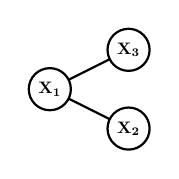
\begin{tikzpicture}[style=thick,scale=1] 
            \begin{scope}[shape=circle,minimum size=0.1cm] 
            \tikzstyle{every node}=[draw,fill] 
            \node[fill=none,scale=\ztnodesize] (X_1) at (0,0.5) {$\mathbf{X_1}$};
            \node[fill=none,scale=\ztnodesize] (X_2) at (1,0) {$\mathbf{X_2}$};
            \node[fill=none,scale=\ztnodesize] (X_3) at (1,1) {$\mathbf{X_3}$};
            \draw [-] (X_1) -- (X_2);
            \draw [-] (X_1) -- (X_3);
            \end{scope} 
        \end{tikzpicture}
        \caption{The Original Undirected Graph}
            \label{fig:utm1}
        \end{center}
\end{figure}

\noindent We can draw the corresponding directed graph as Figure \ref{fig:dtm2}.
\begin{figure}[h]
    \begin{center}
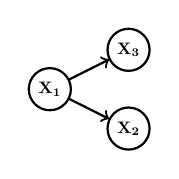
\begin{tikzpicture}[style=thick,scale=1] 
            \begin{scope}[shape=circle,minimum size=0.1cm] 
            \tikzstyle{every node}=[draw,fill] 
            \node[fill=none,scale=\ztnodesize] (X_1) at (0,0.5) {$\mathbf{X_1}$};
            \node[fill=none,scale=\ztnodesize] (X_2) at (1,0) {$\mathbf{X_2}$};
            \node[fill=none,scale=\ztnodesize] (X_3) at (1,1) {$\mathbf{X_3}$};
            \draw [->] (X_1) -- (X_2);
            \draw [->] (X_1) -- (X_3);
            \end{scope} 
        \end{tikzpicture}
        \caption{The Converted Directed Graph}
            \label{fig:dtm2}
        \end{center}
\end{figure}

\noindent This suggests the following factorization of the joint probability:
\begin{eqnarray}
P(X_1, X_2, X_3) = P(X_3 | X_1) P(X_2 | X_1) P(X_1) \nonumber
\end{eqnarray}

Now consider the following graphical model in Figure \ref{fig:utm}.
\begin{figure}[h!]
    \begin{center}
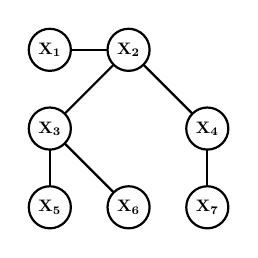
\begin{tikzpicture}[style=thick,scale=1] 
            \begin{scope}[shape=circle,minimum size=0.1cm] 
            \tikzstyle{every node}=[draw,fill] 
            \node[fill=none,scale=\ztnodesize] (X_1) at (0,2) {$\mathbf{X_1}$};
            \node[fill=none,scale=\ztnodesize] (X_2) at (1,2) {$\mathbf{X_2}$};
            \node[fill=none,scale=\ztnodesize] (X_3) at (0,1) {$\mathbf{X_3}$};
            \node[fill=none,scale=\ztnodesize] (X_4) at (2,1) {$\mathbf{X_4}$};
            \node[fill=none,scale=\ztnodesize] (X_5) at (0,0) {$\mathbf{X_5}$};
            \node[fill=none,scale=\ztnodesize] (X_6) at (1,0) {$\mathbf{X_6}$};
            \node[fill=none,scale=\ztnodesize] (X_7) at (2,0) {$\mathbf{X_7}$};
            \draw [-] (X_1) -- (X_2);
            \draw [-] (X_2) -- (X_3);
            \draw [-] (X_2) -- (X_4);
            \draw [-] (X_3) -- (X_5);
            \draw [-] (X_3) -- (X_6);
            \draw [-] (X_4) -- (X_7);
            \end{scope} 
        \end{tikzpicture}
        \caption{An Undirected Graph}
            \label{fig:utm}
        \end{center}
\end{figure}

As before, we can read the conditional independence relations from the graph. 
\begin{enumerate}[label=(\alph*)]
\item Following the example above, write a factorization of the joint distribution into directed, conditional probability distributions:

\begin{center}
$P(X_1,X_2,X_3,X_4,X_5,X_6,X_7)$.
\end{center}

\begin{answertext}{3 cm}{}

\end{answertext}

\item Is this factorization unique, meaning, could you have written other factorizations that correspond this model? If the factorization is unique, explain why it is unique. If it is not unique, provide an alternate factorization.

\begin{answertext}{5 cm}{}

\end{answertext}

\item What is it about these examples that allows them to be factored in this way?

\begin{answertext}{9 cm}{}

\end{answertext}
\end{enumerate}

\newquestion
\section*{\arabic{QuestionCounter}) Generative model and Discriminative model (10 points)}
Consider the graphical model shown in Figure \ref{fig:tree_graph}. In this model, $\vx$ is a sequence of observations for which we want to output a prediction $\vy$, which itself is a sequence, where the size of $\vy$ is the same as $\vx$. Unlike sequence models we discussed in class, this model has a tree structure over the hidden nodes. Assume that the potential functions have a log-linear form: $\psi(Z) = \exp\{\sum_i \theta_i f_i(Z)\}$, where $Z$ is the set of nodes that are arguments to the potential function (i.e. some combination of nodes in $\vx$ and $\vy$,) $\theta$ are the parameters of the potential functions and $f_i$ is a feature function.

\begin{small}
\begin{figure}[h]
    \begin{center}
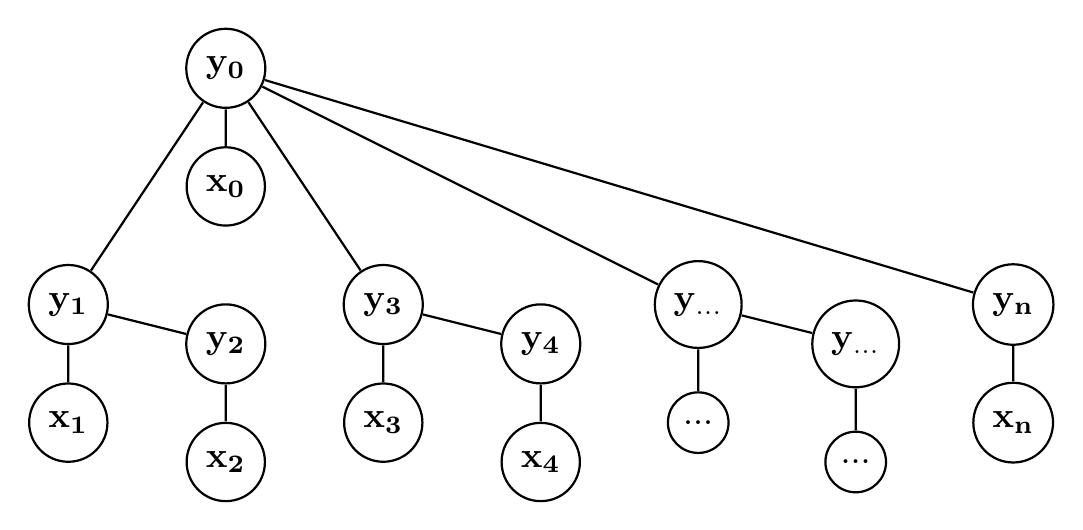
\begin{tikzpicture}[style=thick,scale=1]
            \begin{scope}[shape=circle,minimum size=0.1cm]
            \tikzstyle{every node}=[draw,fill]
            
            \node[fill=none,scale=\nodesize] (y_0) at (2,4.5) {$\mathbf{y_{0}}$};
            \node[fill=none,scale=\nodesize] (X_0) at (2,3) {$\mathbf{x_0}$};
            
            \node[fill=none,scale=\nodesize] (y_1) at (0,1.5) {$\mathbf{y_{1}}$};
            \node[fill=none,scale=\nodesize] (X_1) at (0,0) {$\mathbf{x_1}$};
            \node[fill=none,scale=\nodesize] (y_10) at (2,1.0) {$\mathbf{y_{2}}$};
            \node[fill=none,scale=\nodesize] (X_10) at (2,-0.5) {$\mathbf{x_2}$};
            
            \node[fill=none,scale=\nodesize] (y_2) at (4,1.5) {$\mathbf{y_{3}}$};
            \node[fill=none,scale=\nodesize] (X_2) at (4,0) {$\mathbf{x_3}$};
            \node[fill=none,scale=\nodesize] (y_20) at (6,1.0) {$\mathbf{y_{4}}$};
            \node[fill=none,scale=\nodesize] (X_20) at (6,-0.5) {$\mathbf{x_4}$};
            
            \node[fill=none,scale=\nodesize] (y_3) at (8,1.5) {$\mathbf{y_{\ldots}}$};
            \node[fill=none,scale=\nodesize] (X_3) at (8,0) {$\mathbf{...}$};
            \node[fill=none,scale=\nodesize] (y_30) at (10,1.0) {$\mathbf{y_{\ldots}}$};
            \node[fill=none,scale=\nodesize] (X_30) at (10,-0.5) {$\mathbf{...}$};          
            
            \node[fill=none,scale=\nodesize] (y_4) at (12,1.5) {$\mathbf{y_{n}}$};
            \node[fill=none,scale=\nodesize] (X_4) at (12,0) {$\mathbf{x_n}$};
            
            \draw [-] (X_0) -- (y_0);
            
            \draw [-] (y_0) -- (y_1);
            \draw [-] (X_1) -- (y_1);
            \draw [-] (y_1) -- (y_10);
            \draw [-] (X_10) -- (y_10);
            
            \draw [-] (y_0) -- (y_2);
            \draw [-] (X_2) -- (y_2);
            \draw [-] (y_2) -- (y_20);
            \draw [-] (X_20) -- (y_20);
            
            \draw [-] (y_0) -- (y_3);
            \draw [-] (X_3) -- (y_3);
            \draw [-] (y_3) -- (y_30);
            \draw [-] (X_30) -- (y_30);
            
            \draw [-] (y_0) -- (y_4);
            \draw [-] (X_4) -- (y_4);
            
            \end{scope}
        \end{tikzpicture}
            \caption{Tree structure model}
            \label{fig:tree_graph}
        \end{center}
\end{figure}
\end{small}
\begin{enumerate}[label=(\alph*)]
\item Write the log likelihood for this model of a single instance $\vx$: $\log{p(\vy,\vx)}$. 

\begin{answertext}{6 cm}{}

\end{answertext}
\newpage
\item Write the conditional log likelihood for this model of a single instance $\vx$: $\log{p(\vy|\vx)}$. 

\begin{answertext}{6 cm}{}

\end{answertext}
\item Assume that each variable $y_i$ can take one of $k$ possible states, and variable $x_i$ can take one of $k'$ possible states, where $k'$ is very large. Describe the computational challenges of modeling $\log p(\vy,\vx)$ vs $\log p(\vy|\vx)$.

\begin{answertext}{6 cm}{}

\end{answertext}
\item Propose an efficient algorithm for making a prediction for $\vy$ given $\vx$ and $\theta$.

\begin{answertext}{4 cm}{}

\end{answertext}
\end{enumerate}



\newquestion
\section*{\arabic{QuestionCounter}) Sequence Classification (10 points)}
Consider the following sequence classification task. We are given sequences of words, and only three words can appear in a sequence: ``dog'', ``cat'', ``stop''. The sequences can be arbitrarily long, but every sequence must end with the word ``stop''. 

We want to fit a sequence model to this data, where there is a hidden state corresponding to each observed word. When we are given a sequence, we infer the hidden states according to the pre-trained model parameters. We use the final state (corresponding to the last word ``stop'') and use it to predict whether of not the sequence was {\sc good} or {\sc bad}. You can make this prediction by either examining the final state itself, or using the final state as input to a classifier that predicts {\sc good} or {\sc bad}.

A {\sc good} sequence is one in which the words ``dog'' and ``cat'' appear an equal number of times (including 0 times.) A {\sc bad} sequence is every other sequence.

For example:
\begin{quote}
\begin{verbatim}
dog cat dog dog dog dog cat stop
\end{verbatim}
 ({\sc bad})
\end{quote}

\begin{quote}
\begin{verbatim}
cat cat cat cat cat stop cat cat cat cat stop
\end{verbatim}
 ({\sc bad})
\end{quote}

\begin{quote}
\begin{verbatim}
cat cat dog cat cat stop dog dog dog cat cat dog dog stop
\end{verbatim}
 ({\sc good})
\end{quote}

You may use as much training data as you'd like, or manually set the model parameters yourself.

For each of the following sequence models, state as to whether there exist model parameters that can accurately capture the desired behavior. Explain why.

\begin{enumerate}[label=(\alph*)]
\item Hidden Markov Model

\begin{answertext}{8 cm}{}

\end{answertext}
\item Conditional Random Field

\begin{answertext}{8 cm}{}

\end{answertext}
\item Recurrent Neural Network

\begin{answertext}{8 cm}{}

\end{answertext}
\end{enumerate}

\end{document}
